\documentclass[a4paper,12pt]{article}

% --- Math and Base Packages ---
\usepackage{amsmath}
\usepackage{amssymb} % Provides \geqslant and other symbols
\usepackage{graphicx}
\usepackage[left=2.5cm,right=2.5cm,top=2cm,bottom=2cm]{geometry}

% --- Font Configuration (XeLaTeX) ---
\usepackage{fontspec}
\usepackage{polyglossia}
\setmainlanguage{english}

\setmainfont{Libertinus Sans}
\setmonofont{IBM Plex Mono}[Scale=MatchLowercase]

% Match Math Style to the Main Sans Font
\usepackage[italic]{mathastext}

% --- Graphics and Layout ---
\usepackage{tikz}
\usetikzlibrary{arrows.meta,positioning,fit,calc}
\usepackage{cellspace}
\setlength\cellspacetoplimit{4pt}
\setlength\cellspacebottomlimit{4pt}
\usepackage{csquotes}
\usepackage{indentfirst}
\usepackage{listings}

\usepackage{setspace}
\setstretch{1.1}

% --- Code Listings Setup ---
\lstset{
    basicstyle=\ttfamily\small\color{black!85},
    columns=flexible,
    keepspaces=true,
    aboveskip=1em,
    belowskip=1em,
    xleftmargin=1.5em
}

\tikzset{
    recordbox/.style={
        draw,
        inner xsep=6pt,
        inner ysep=4pt,
        outer sep=0pt,
        align=center
    },
    recorddot/.style={
        draw,
        inner sep=2pt,
        minimum width=1.2em,
        outer sep=0pt,
        align=center
    }
}
\makeatletter
\pgfkeys{/tikz/minimumheight/.code=\pgfkeysalso{/tikz/minimum height=#1}}
\pgfkeys{/tikz/minimumwidth/.code=\pgfkeysalso{/tikz/minimum width=#1}}
\makeatother
\sloppy

% --- Информация о статье ---
% --- Article Information ---
\title{Apogee Object Storage Architecture}
\author{Denis Cheremisov}
\date{\today}

\begin{document}

    \maketitle

    \begin{abstract}
        This paper describes the architecture of an object storage system designed for scalability, high local and
        global performance, and superior diagnosability. These goals are achieved through a simplified component
        interaction model, where each component is strictly isolated within its own domain of responsibility.
    \end{abstract}

    \newpage
    \tableofcontents

    \newpage  % необязательно


    \section{Definitions}

    The system is composed of the following components:

    \begin{itemize}
        \item \textbf{Stateless Coordinators.}

        \item \textbf{Cold Storage (Cold Tier)}, which consists of cold nodes:
        \begin{itemize}
            \item A RAFT-based allocator for managing tuples and allocating \textit{stripes} within them.
            \item Disk tuples managed by the allocator.
        \end{itemize}

        \item \textbf{Heat (Hot Tier)}, represented by hot nodes consisting of three machines in an identical configuration. Multiple hardware variants are possible depending on cost and performance requirements.

        \item \textbf{WAL (Write-Ahead Log)}: A distributed WAL. Currently, the simplest implementation uses a message broker and a KV store with persistence and consistency guarantees (e.g., NATS + JetStream, providing both broker and KV functionality).

        \item \textbf{Metadata}:
        \begin{itemize}
            \item \textbf{Records}: Stores metadata for user records.
            \item \textbf{Fragments}: Stores metadata for data fragments, including fields for deduplication support.
            \item \textbf{Links}: A collection mapping Records to Fragments.
            \item \textbf{Containers}: Describes the physical placement of fragment containers. A container can be either \enquote{sealed} within a cold tier stripe or temporarily reside in a hot tier buffer.
            \item \textbf{Tuples}: Links cold tier tuples to physical disks.
        \end{itemize}
    \end{itemize}


    \newpage


    \section{Physical System Design}

    \subsection{Hot Storage Layer}

    I propose three distinct approaches here, varying in hardware exoticism and cost. In all cases, the hot layer employs the maximum degree of redundancy. At this stage, it is most efficient to work from the \enquote{greatest common denominator}—specifically, using a $3\times$ replication scheme—and then reduce the redundancy level once the data moves to cold storage. Thus, when we refer to a \enquote{hot node}, we mean a set of three physical nodes, each storing a replica of the data. Consequently, the corresponding drives on these machines must be equivalent in terms of hardware LBA and capacity.

    In any mode, a disk $D_i$ is represented as follows:

    \begin{gather*}
        D_i = \left(B_{i1}, B_{i2}, \dots, B_{im}\right)\\
        |B_{i1}| = |B_{i2}| = \dots = |B_{im}| = 64\text{MiB}\\
    \end{gather*}

    The blocks $B_{ij}$ are referred to as \textit{buffers}.

    \subsubsection{Maximum Performance Mode}

    Hardware requirements:

    \begin{itemize}
        \item One or more NVMe SSDs.
        \item NVDIMM module(s) (offering similar guarantees to Optane but at a lower cost).
    \end{itemize}

    In this mode, we utilize NVMe SSDs—one, two, or three. Using more is rarely practical, as three drives will saturate any network, and a single NVMe on PCIe Gen5 can saturate it alone.

    \smallskip
    For each disk $D_i$, a memory region $M_i$ is allocated on the NVDIMM modules. This region is likewise divided into equal fragments $M_{ij}$, where $j = 1, 2, \dots, m$:

    \begin{gather*}
        M_i = \left(M_{i1}, M_{i2}, \dots, M_{im}\right)\\
        |M_{i1}| = |M_{i2}| = \dots = |M_{im}|\\
    \end{gather*}

    \begin{center}
        \begin{tikzpicture}[
            block/.style={
                draw,
                minimum width=18mm,
                minimum height=8mm,
                align=center
            },
            rowlabel/.style={
                align=right,
                minimum height=8mm
            },
            container/.style={
                draw,
                rounded corners,
                inner sep=6mm
            },
            node distance=6mm
        ]

            % --- Row label for D_i ---
            \node[rowlabel] (Dl) {$D_i:$};

            % --- Blocks B_ij (disk) ---
            \node[block, right=10mm of Dl] (B1) {$B_{i1}$};
            \node[block, right=of B1] (B2) {$B_{i2}$};
            \node[right=of B2] (Bdots) {$\dots$};
            \node[block, right=of Bdots] (Bm) {$B_{im}$};

            \node[
                container,
                fit=(B1)(B2)(Bdots)(Bm)
            ] (Drow) {};

            % --- Row label for M_i ---
            \node[rowlabel, below=14mm of Dl] (Ml) {$M_i:$};

            % --- Fragments M_ij (memory) ---
            \node[block, right=10mm of Ml] (M1) {$M_{i1}$};
            \node[block, right=of M1] (M2) {$M_{i2}$};
            \node[right=of M2] (Mdots) {$\dots$};
            \node[block, right=of Mdots] (Mm) {$M_{im}$};

            \node[
                container,
                fit=(M1)(M2)(Mdots)(Mm)
            ] (Mrow) {};

            % --- Alignment guides ---
            \foreach \b/\m in {B1/M1,B2/M2,Bm/Mm} {
                \draw[dashed, gray] (\b.south) -- (\m.north);
            }
        \end{tikzpicture}
    \end{center}

    The size of the fragments $M_{ij}$ is determined by the physical block size of the disks. Each $M_{ij}$ stores:

    \begin{itemize}
        \item Metadata for the container currently being filled (or already filled) in buffer $B_{ij}$.
        \item A buffer in the sense of buffered I/O for LBAs not yet filled during a write operation.
    \end{itemize}
    Subsequent writes will fill this buffer, after which it is flushed to the tail of $B_{ij}$.

    Note the strategy for selecting write buffers: we move sequentially from the beginning of the disk to the end. This ensures that all $B_{ij}$ blocks are filled nearly sequentially, providing uniform wear leveling for the storage medium. In the event of a failed write, no attempt should ever be made to rewrite to the same block. Such an attempt would constitute an overwrite, resulting in unnecessary disk wear. Instead, we simply skip the LBA range intended for that fragment. Fundamentally, we strictly adhere to an \textbf{append-only semantics}.

    \smallskip
    This approach enables the system to handle hundreds of high-definition video streams simultaneously.

    \subsubsection{High Performance Mode}

    This mode is similar to the previous one but operates without NVDIMM. In this scenario, buffer metadata is stored in an external database, but LBA-level packing is not performed. Specifically, if a write does not completely fill a storage block, the remainder of the block is zero-filled (padded with zeros), and the subsequent write begins at the start of the next block.

    Overall, this approach provides high performance, though it is inferior to the NVDIMM-based variant. It is less suited for video streaming, as it would require handling LBA-level buffering on the coordinators. This is clearly suboptimal, as it would require the coordinators to have intimate knowledge of the \enquote{Hot Tier internals} (the \enquote{guts} of the Heat layer).

    \subsubsection{Budget On-Premise Solution}

    Disk as a circular buffer.
    \smallskip

    In this mode, we do not attempt any dense packing of buffers. If a written fragment exceeds the current buffer boundaries, the buffer is immediately sealed and prepared for migration to the Cold Tier, while the fragment is written to the next available buffer. This approach is ill-suited for streaming; thus, this type of Heat layer is only appropriate for document stores and similar workloads. However, it is highly cost-effective and can be implemented on any hardware, including HDDs.

    \subsection{Cold Storage Layer}

    The Cold Tier is divided into cold nodes, each consisting of a pair:
    \begin{itemize}
        \item A RAFT-based allocator.
        \item A set of disk tuples.
    \end{itemize}

    A tuple $T$ is defined as a set of disks:
    \[T=\left( D_1, D_2, \dots, D_N \right)\]
    The disks themselves are represented as sets of blocks of uniform size:
    \[D_i = \left( C_{i1}, C_{i2}, \dots, C_{iM} \right)\]
    A \textit{stripe} $S_j$ within tuple $T$ is defined as the set of blocks with index $j$ collected from all disks in the tuple:
    \[S_j = \left( C_{1j}, C_{2j}, \dots, C_{Nj} \right)\]

    The primary task of the RAFT allocator is to locate free stripes within the managed tuples. Specifically, it first selects a tuple and then searches for an available stripe. Tracking of free and occupied stripes is performed using a tuple \textit{bitmap}, where each stripe is mapped to a bit: 1 for occupied and 0 for free.

    \begin{center}
        \begin{tikzpicture}[
            block/.style={
                draw,
                minimum width=2.2cm,
                minimum height=1.2cm,
                align=center
            },
            stripe/.style={
                dashed,
                gray
            },
            vsep/.style={
                dashed,
                very thick,
                gray
            },
            bitone/.style={
                draw,
                fill=black,
                minimum width=1.0cm,
                minimum height=1.0cm
            },
            bitzero/.style={
                draw,
                fill=white,
                line width=1pt,
                minimum width=1.0cm,
                minimum height=1.0cm
            }
        ]

            % Parameters
            \def\ndisks{3}
            \def\nstripes{5}

            % --- Bitmap definition: 1 = occupied, 0 = free ---
            \def\bitmap{1,1,0,1,0}

            % Layout parameters
            \def\xDiskStep{3}
            \def\yStripeStep{1.4}
            \def\xLabel{0.8}
            \def\xStripeLineL{1.2}
            \def\xStripeLineR{10}

            % Bitmap column x positions
            \def\xSep{11.2}     % vertical separator x
            \def\xBmp{12.2}     % bitmap squares x

            % Disk labels
            \foreach \i in {1,...,\ndisks} {
                \node at (\i*\xDiskStep, -0.2) {\textbf{Disk $D_{\i}$}};
            }

            % Blocks C_ij
            \foreach \i in {1,...,\ndisks} {
                \foreach \j in {1,...,\nstripes} {
                    \node[block] (c\i\j) at (\i*\xDiskStep, -\j*\yStripeStep) {$C_{\i\j}$};
                }
            }

            % Stripe separators, labels, and bitmap squares
            \foreach[count=\j from 1] \b in \bitmap {

            % horizontal dashed stripe line
                \draw[stripe] (\xStripeLineL, -\j*\yStripeStep+0.7) -- (\xStripeLineR, -\j*\yStripeStep+0.7);

            % stripe label: S_j (occupied/free)
                \ifnum
                    \b=1
                    \node[anchor=east] at (\xLabel, -\j*\yStripeStep) {$S_{\j}$ (occupied)};
                \else
                    \node[anchor=east] at (\xLabel, -\j*\yStripeStep) {$S_{\j}$ (free)};
                \fi

            % bitmap square
                \ifnum
                    \b=1
                    \node[bitone]  at (\xBmp, -\j*\yStripeStep) {};
                \else
                    \node[bitzero] at (\xBmp, -\j*\yStripeStep) {};
                \fi
            }

            % Bitmap title
            \node[anchor=west] at (\xBmp-0.6, -0.2) {\textbf{Bitmap}};

            % Vertical dashed separator
            \draw[vsep]
            (\xSep, -1*\yStripeStep+0.9) -- (\xSep, -\nstripes*\yStripeStep-0.9);

        \end{tikzpicture}
    \end{center}

    Stripe allocation is performed in two steps:

    \begin{enumerate}
        \item Stripe \textbf{Lease}.
        \item Confirmation of occupation (\textbf{Commit}) or cancellation (\textbf{Release}).
    \end{enumerate}

    A \textit{Release} is triggered automatically via TTL if no signal is received from the coordinator managing the migration within $\Delta$ seconds. Thus, moving 64\,MiB of data requires only 2 RAFT operations. This scales to 64 RAFT operations per second for a aggregate data flow of 2\,GiB/s. This overhead is negligible, especially considering that latency is not a primary concern for this background process.

    \subsection{Tuple Selection}

    When selecting a tuple, the goal is to favor those that are the least filled and not currently over-utilized. The following algorithm should be effective for this purpose.

    Given a parameter $N$ (a natural number), tuples are stored in the following structure:
    \begin{lstlisting}
    tuples = RBTree[FreeStripes, LinkedList[Tuple]]
    \end{lstlisting}
    This means tuples are grouped by the number of available stripes they contain and are ordered by this count. Stripe selection for a write operation proceeds as follows:
    \begin{enumerate}
        \item Select a random $K$ from the range $\left[ 0, N \right)$.
        \item Retrieve the $K$-th tuple from the structure and initiate the data write process.
        \item Upon confirmation of the write, remove the tuple from its current linked list and move it to the end of the list corresponding to the new (lower) free stripe count.
    \end{enumerate}
    Highly loaded tuples can be skipped and ignored during the search for the $K$-th element. While this increases search complexity, the overhead remains minimal, as we are only performing approximately 32 such operations per 2\,GiB/s of throughput.

    \subsection{Metadata}

    TiKV is the most suitable database for metadata storage, offering virtually unlimited horizontal scalability and high performance, particularly in \texttt{rawkv} mode.

    \subsubsection{Records}

    \noindent
    \begin{tabular}{|Sl|Sc|Sc|Sr|}
        \hline
        record.id & single & fragment.id & $\dots$ \\
        \hline
    \end{tabular}

    \bigskip

    \noindent
    \begin{tabular}{|Sl|Sc|Sc|Sr|}
        \hline
        record.id & multi & no\_of\_fragments & $\dots$ \\
        \hline
    \end{tabular}

    \bigskip
    This collection stores record metadata. For records consisting of a single fragment, we store the reference directly within the \textit{Records} entry to avoid redundant storage. In scenarios involving small object storage, this optimization results in a $1.5\times$ reduction in the number of metadata entries by eliminating the need for \textit{Links} records.

    \subsubsection{Fragments}

    \noindent
    \begin{tabular}{|Sl|Sc|Sc|Sc|Sc|Sc|Sc|Sc|Sr|}
        \hline
        fragment.id & container.id & offset & size & crc64 & compression type & blake3 & $\dots$ \\
        \hline
    \end{tabular}

    \bigskip
    Stores fragment metadata.

    \subsubsection{Links}

    \noindent
    \begin{tabular}{|Sl|Sc|Sc|Sr|}
        \hline
        record.id & fragment.index & fragment.id \\
        \hline
    \end{tabular}

    \bigskip
    Stores mappings between records and fragments:
    \bigskip

    \noindent
    \begin{tabular}{|Sl|Sc|Sc|Sr|}
        \hline
        rid & 0     & $\operatorname{fid}_0$ \\
        \hline
        rid & 1     & $\operatorname{fid}_1$ \\
        \hline
        rid & 2     & $\operatorname{fid}_2$ \\
        \hline
        & \dots &                        \\
        \hline
        rid & n     & $\operatorname{fid}_n$ \\
        \hline
    \end{tabular}

    \bigskip
    In practice, it is more efficient to store $\operatorname{SPECK128}(i)$ instead of sequential indices $0, 1, \dots$. This prevents hotspots where a single shard receives a disproportionate number of entries from records with many fragments. By employing this deterministic permutation, entries are uniformly distributed across shards. While this sacrifices the ability to perform range scans for sequential fragment retrieval, this is not a significant drawback: since all fragments (except the last) are approximately 64\,MiB, metadata retrieval speed will not become a bottleneck.

    Consequently, the iteration logic changes from:
    \begin{lstlisting}
for x in records_fragments_iterator:
  read_fragment(x.fragment_id)
    \end{lstlisting}
    to:
    \begin{lstlisting}
for i in [0, record.no_of_fragments):
  fragment_id := records_fragments.get_fragment(record.id, speck128(i))
  read_fragment(fragment_id)
    \end{lstlisting}

    \subsubsection{Containers}

    \noindent
    \begin{tabular}{|Sl|Sr|}
        \hline
        container.id & ref \\
        \hline
    \end{tabular}

    \bigskip
    Where \texttt{ref} can be either \texttt{Hot(hot.id, block.index)} or \texttt{Tuple(tuple.id, stripe.index)}.

    \subsubsection{Tuples}

    \noindent
    \begin{tabular}{|Sl|Sr|}
        \hline
        tuple.id & payload \\
        \hline
    \end{tabular}

    \bigskip
    The \texttt{payload} is structured as follows:
    \begin{lstlisting}
    {
        type: encoding scheme used (e.g., Replication or EC)
        disks: [
            (disk1, role1),
            ...
            (diskN, roleN),
        ]
    }
    \end{lstlisting}


    \newpage


    \section{Processes}

    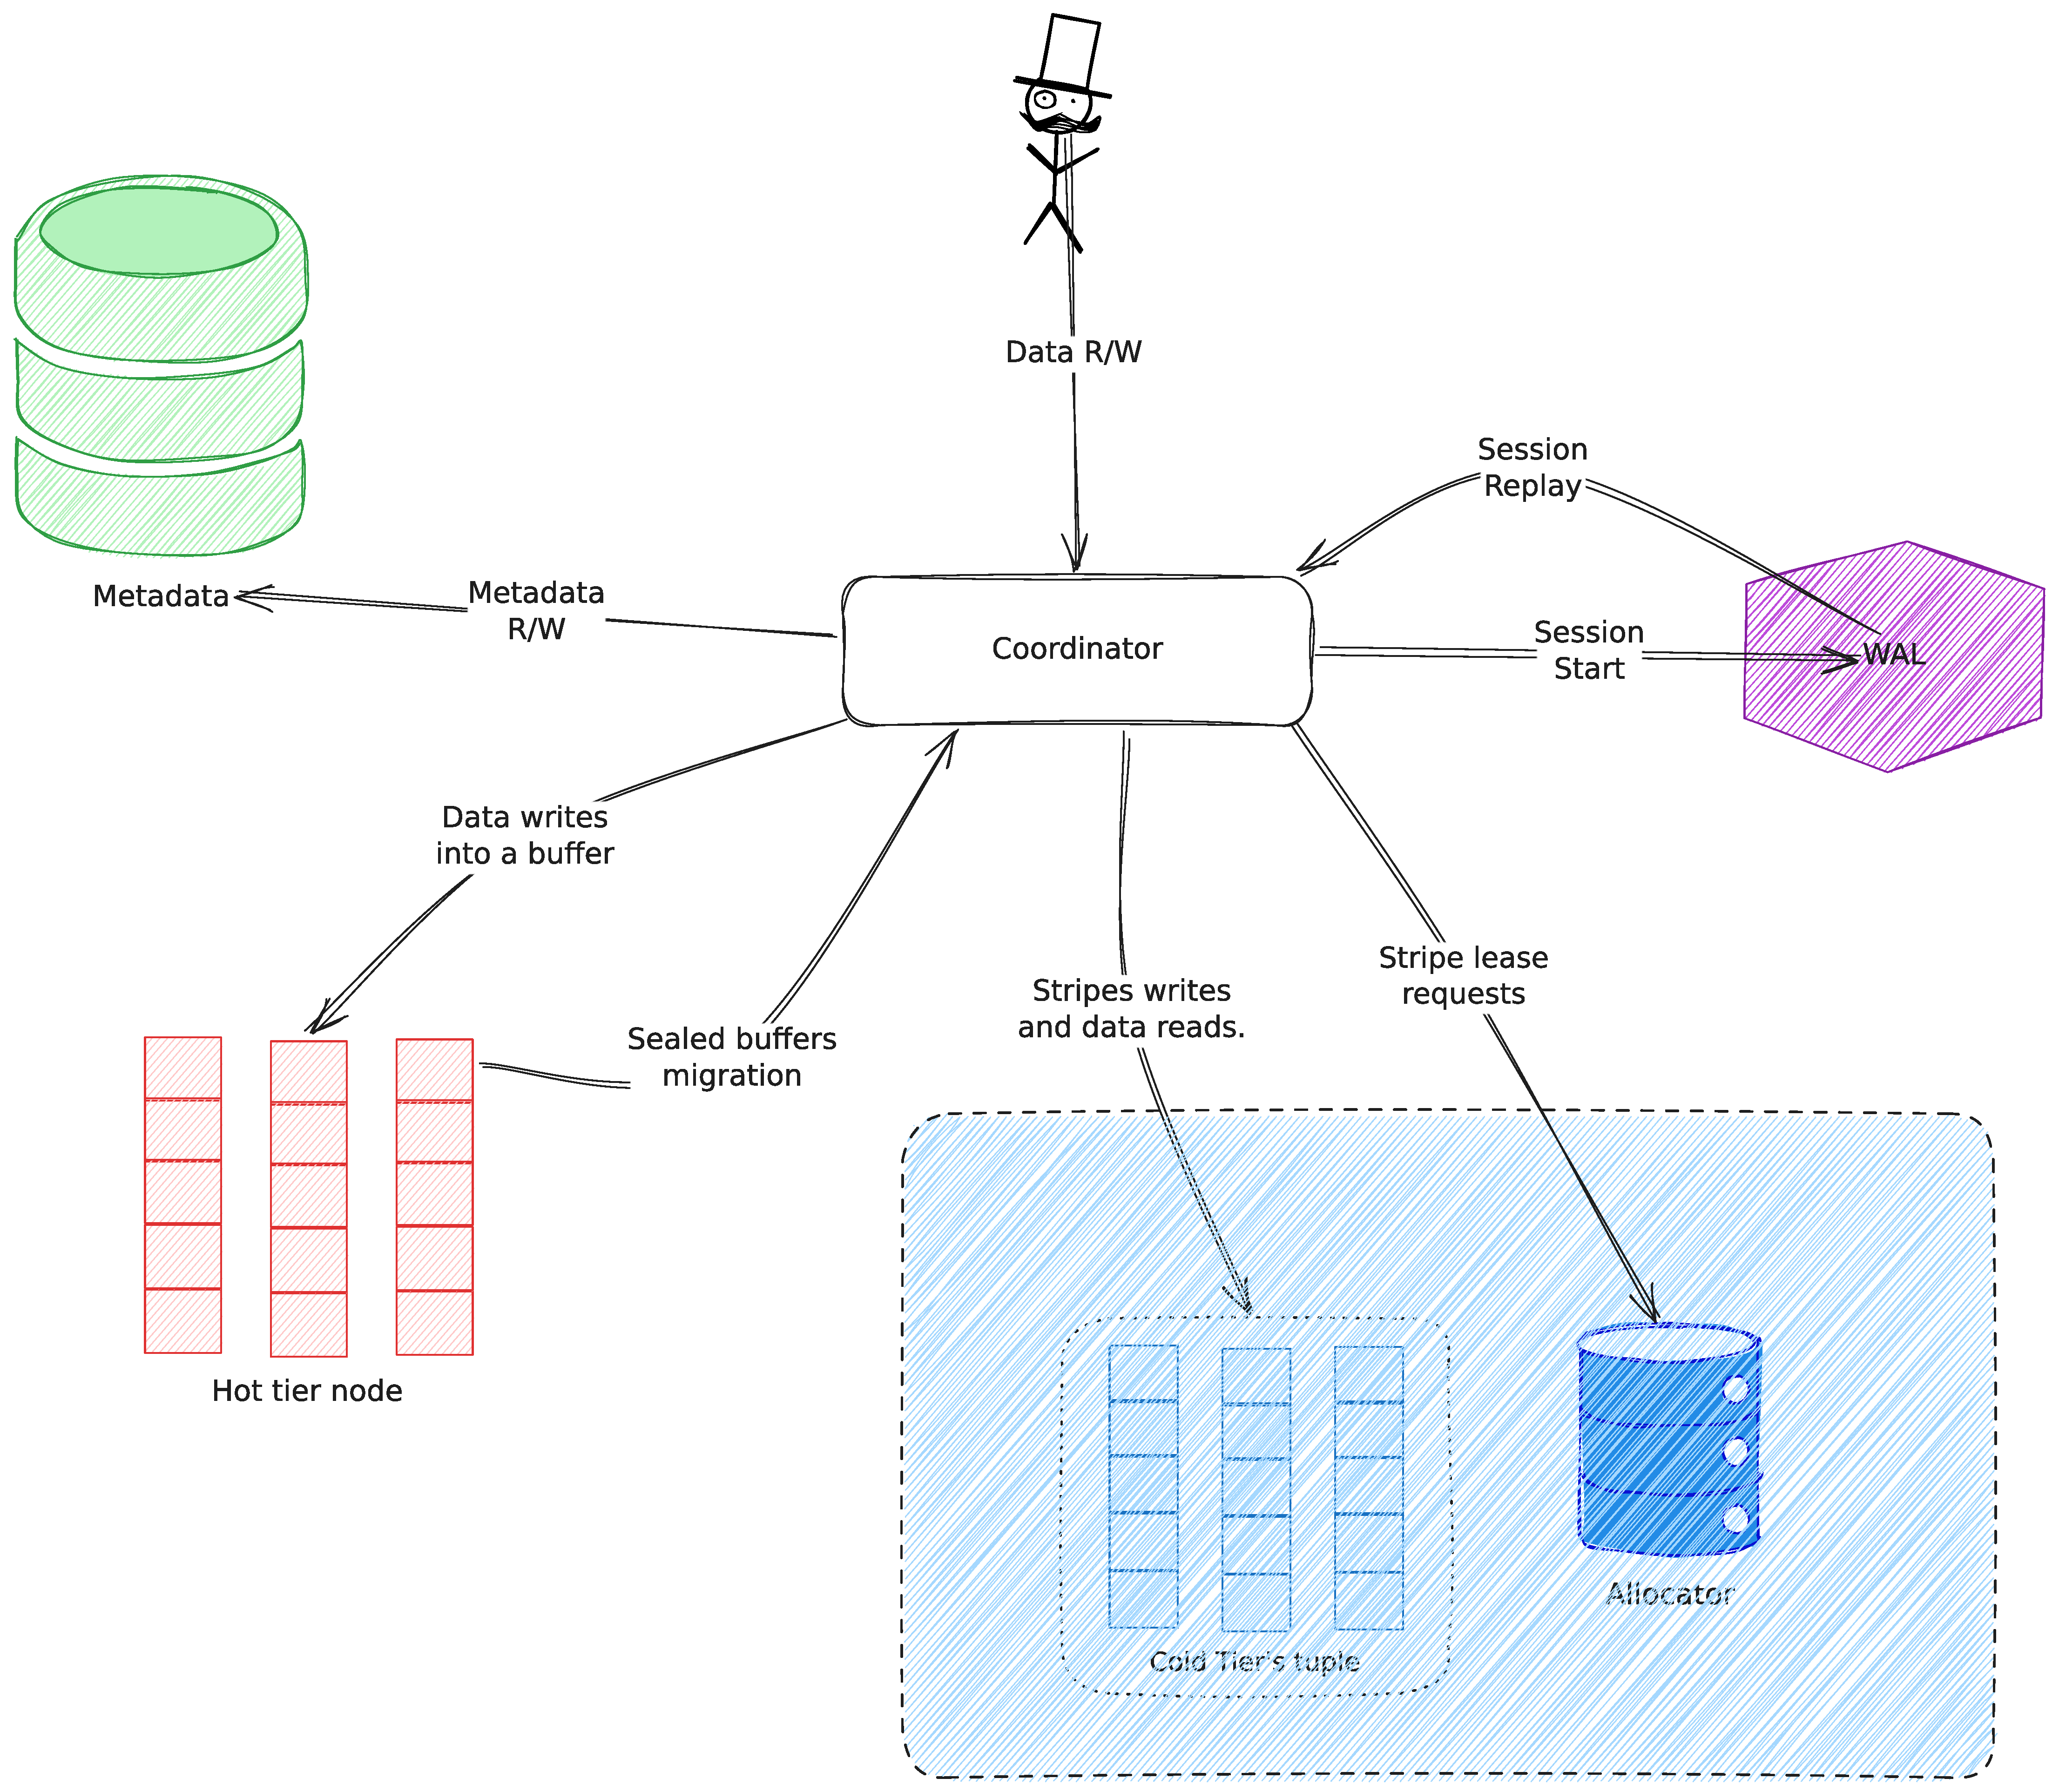
\includegraphics[width=\linewidth]{resources/arch-en}

    \subsection{High-Level Overview}

    Broadly speaking, the system's operational logic is as follows:

    \subsubsection{Write Path}

    \begin{enumerate}
        \item The client \textbf{streams} data to the coordinator.
        \item The coordinator \textbf{chunks} the stream into fragments, writes them to the \textit{Heat} layer, and records the corresponding metadata in the metadata database.
        \item The coordinator returns a \textit{Record ID} to the client.
    \end{enumerate}

    Writing to the \textit{Heat} layer triggers periodic signals that initiate data migration from \textit{Heat} to \textit{Cold}:

    \begin{enumerate}
        \item The \textit{Heat} layer notifies the \textbf{migrator} (which may reside within a coordinator) that a buffer is ready for transfer.
        \item The migrator pulls the data from \textit{Heat}, locates an available stripe in the \textit{Cold} tier, writes the data, and subsequently updates the metadata database to reflect the new physical location.
    \end{enumerate}

    \subsubsection{Read Path}

    \begin{enumerate}
        \item The client requests record data from the coordinator.
        \item The coordinator queries the metadata database to locate the data and reads from the \textit{Cold Tier} and/or \textit{Hot Tier} accordingly.
    \end{enumerate}

    \subsection{Index Generation}

    An \textit{etcd} instance is used to store \texttt{u128} counters for \texttt{record.id}, \texttt{fragment.id}, \texttt{container.id}, etc. Upon startup, a coordinator requests a range of IDs from \textit{etcd} (e.g., $2^{20}$ values) and then allocates them locally one by one.

    To ensure uniform distribution across shards, we use the \texttt{SPECK128(id)} encoded value rather than the raw identifier. This provides a high-quality uniform distribution. While an alternative would be adding a \texttt{hash(id)} column to the tables, this would incur additional storage overhead. \texttt{SPECK128} is a superior choice as it achieves the same goal without extra metadata.

    \subsection{Deduplication}

    Fragment data includes the following fields:

    \begin{center}
        \begin{tabular}{|Sl|Sc|Sc|Sr|}
            \hline
            CRC64 & Size & CompressionType & Blake3 \\
            \hline
        \end{tabular}
    \end{center}

    \bigskip
    We maintain a deduplication collection with the following schema:

    \begin{center}
        \begin{tabular}{|Sl|Sc|Sc|Sc|Sc|Sr|}
            \hline
            CRC64 & Size & CompressionType & Blake3 & fragment.id & epoch \\
            \hline
        \end{tabular}
    \end{center}

    \bigskip
    During a fragment write, we check this collection for existing matches. If a match is found, we evaluate its \textit{epoch}:

    \begin{itemize}
        \item If the epoch is too far in the past, the existing fragment is ignored; we write a new fragment and update the deduplication record with the new reference.
        \item Otherwise, we skip the data write and reference the existing fragment.
    \end{itemize}

    This procedure may occasionally lead to minor data duplication due to race conditions (e.g., two concurrent processes writing the same fragment and updating the deduplication entry simultaneously). However, this is largely an \textit{edge case}. In real-world scenarios, such occurrences should be extremely rare, and a scenario leading to significant storage bloat is purely theoretical.

    \subsection{Regular Data Upload Process}

    During a regular upload, where the user provides a dataset of a known size, the entire record $R$ is partitioned into fragments:

    \[R = \left(F_1, F_2, \dots, F_n\right)\]
    where the lengths of all fragments are strictly identical, except for the last one, which may be smaller. Formally:

    \[|F_1| = |F_2| = \dots = |F_{n-1}| \geq |F_{n}|\]
    This constraint is enforced to simplify the support for \textbf{range reads} (reads with an offset). While it is possible to split fragments into blocks of arbitrary sizes, doing so would significantly increase the implementation complexity and cost.

    When a user submits data—simplified here, as the actual process involves WAL operations and a specific sequence of metadata database queries—the following occurs:

    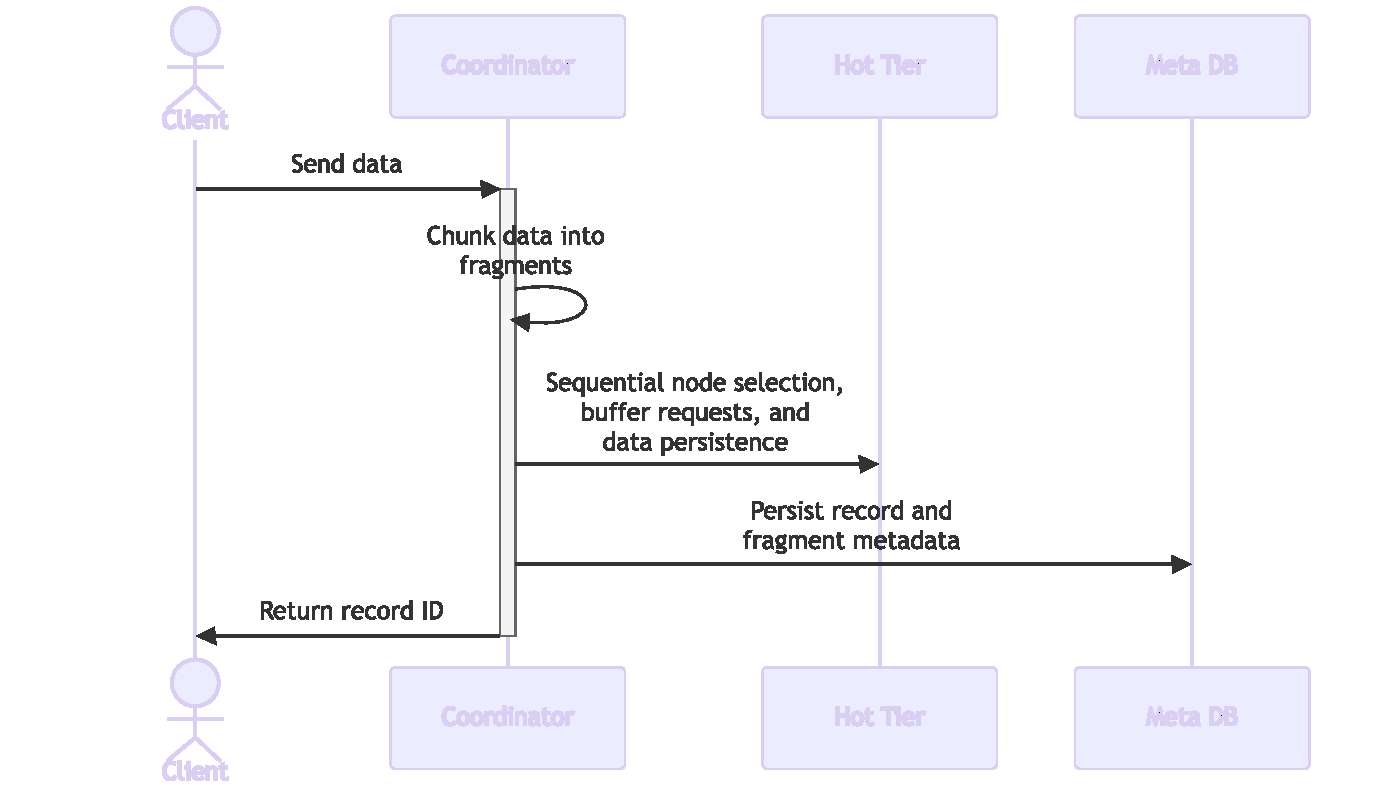
\includegraphics[width=\linewidth]{resources/simple-write-en}

    A complete, formal WritePath sequence, including commit and rollback support, is provided in the Appendices.

    \subsection{Streaming Data Upload Process}

    In this mode, we acquire temporary ownership of a buffer in the \textit{Heat} layer with a confirmation. Data is then streamed into this buffer until it is full. Once filled, the buffer is \textbf{sealed}, and a task is queued for its migration to the \textit{Cold Tier}.

    A key distinction from the regular upload process is the fragment management: the fragment's status in the \textit{Fragments} collection is marked as \enquote{in progress}, and some of its metadata (such as current size) is stored within the buffer's own metadata. This optimization is necessary to avoid excessive write pressure on the metadata database during the streaming process.

    \subsection{Read Process}

    The system supports both full reads and range reads (reads with an offset). The workflow is as follows:

    \begin{enumerate}
        \item Retrieve the \textit{Record} entry using the provided \texttt{RecordID}.
        \item Retrieve fragment identifiers by scanning the \textit{Links} collection using the key prefix \texttt{(RecordID, <fragment\_index>)}.
        \item For each fragment, fetch its metadata from the \textit{Fragments} collection to identify the corresponding \texttt{ContainerID}.
        \item Retrieve the container's metadata from \textit{Containers} via the \texttt{ContainerID} to determine its physical placement (Heat or Cold tier).
        \item If the container resides in the \textit{Heat} layer, initiate a read request from the corresponding \textit{Heat} buffer.
        \item If the container is in the \textit{Cold} tier (addressed via \texttt{TupleID} and \texttt{StripeIndex}), retrieve the tuple data from \textit{Tuples} and calculate the required blocks based on the fragment's offset within the container.
    \end{enumerate}

    \subsection{Migration from Heat to Cold}

    When a buffer reaches a state where further filling is inefficient due to insufficient free space, the \textit{Heat} layer initiates a migration procedure by invoking the \textbf{migrator}. This process follows the schema below:

    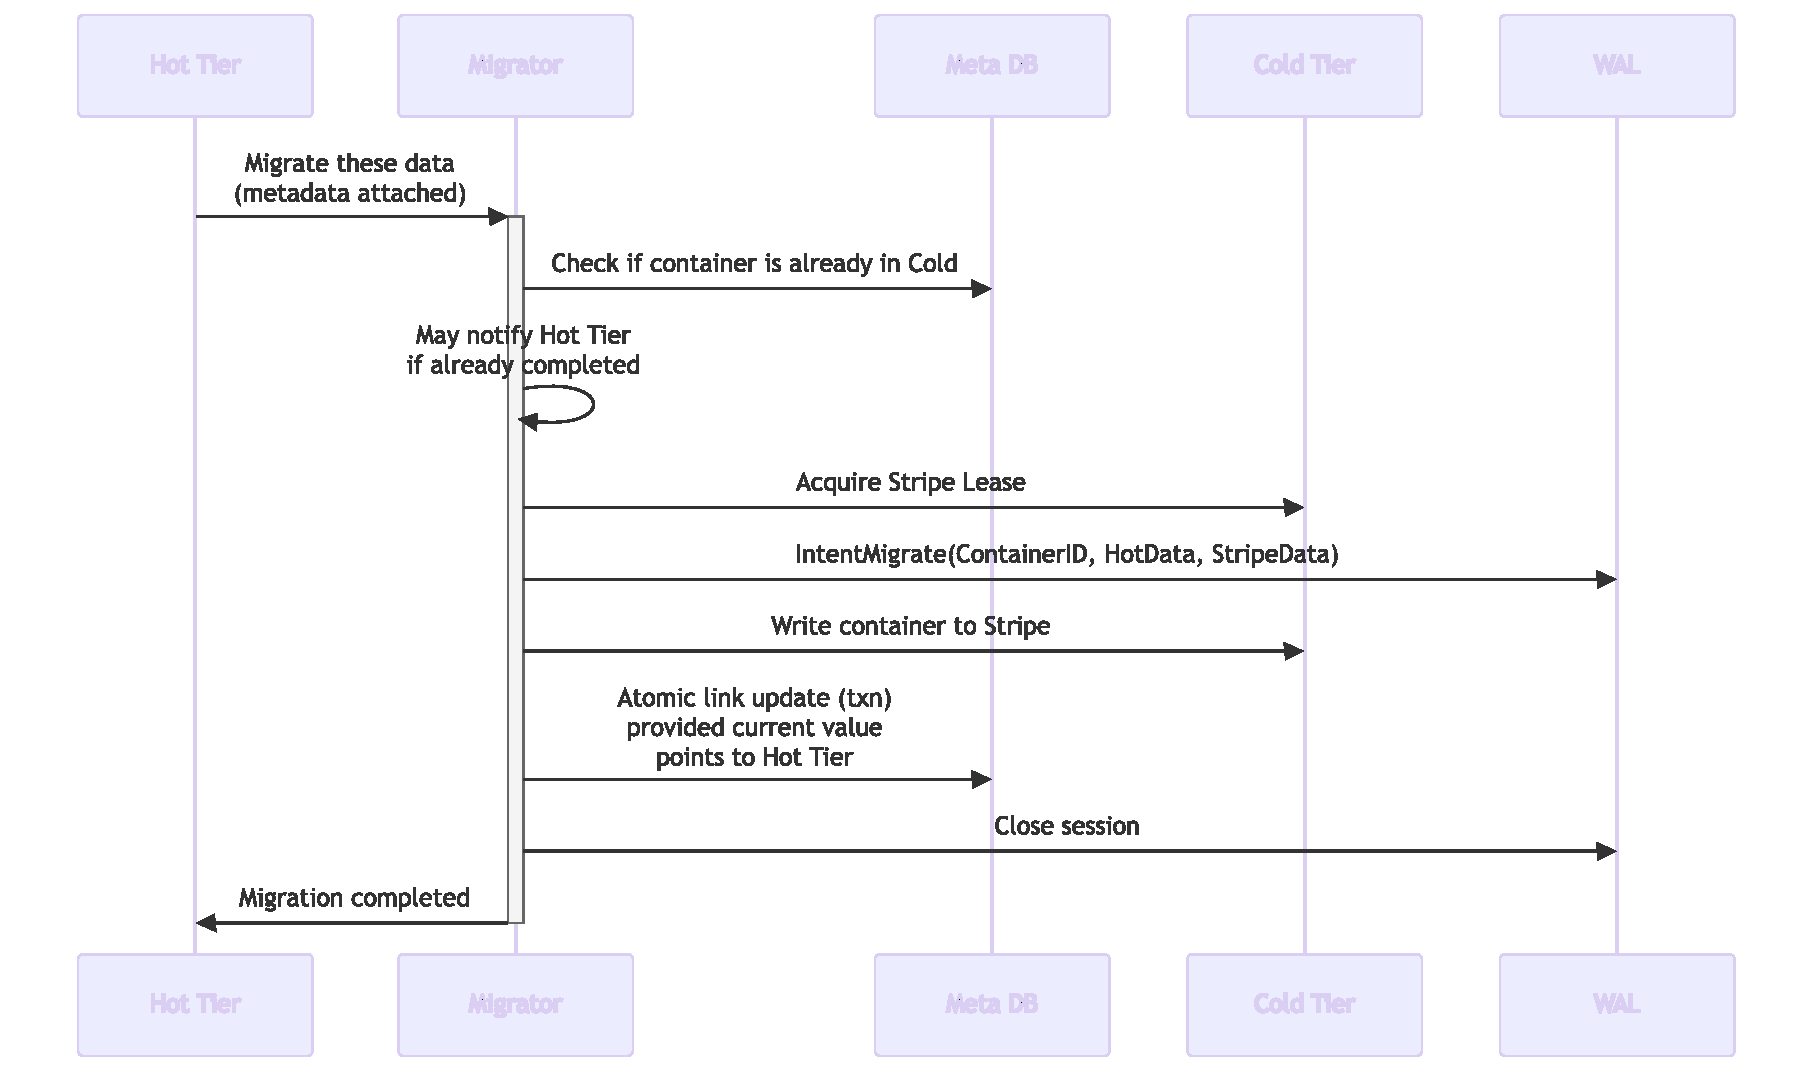
\includegraphics[width=\linewidth]{resources/migration-en}

    The use of transactions is mandatory to prevent the creation of \textbf{orphaned resources}, as illustrated in the following collision scenario:

    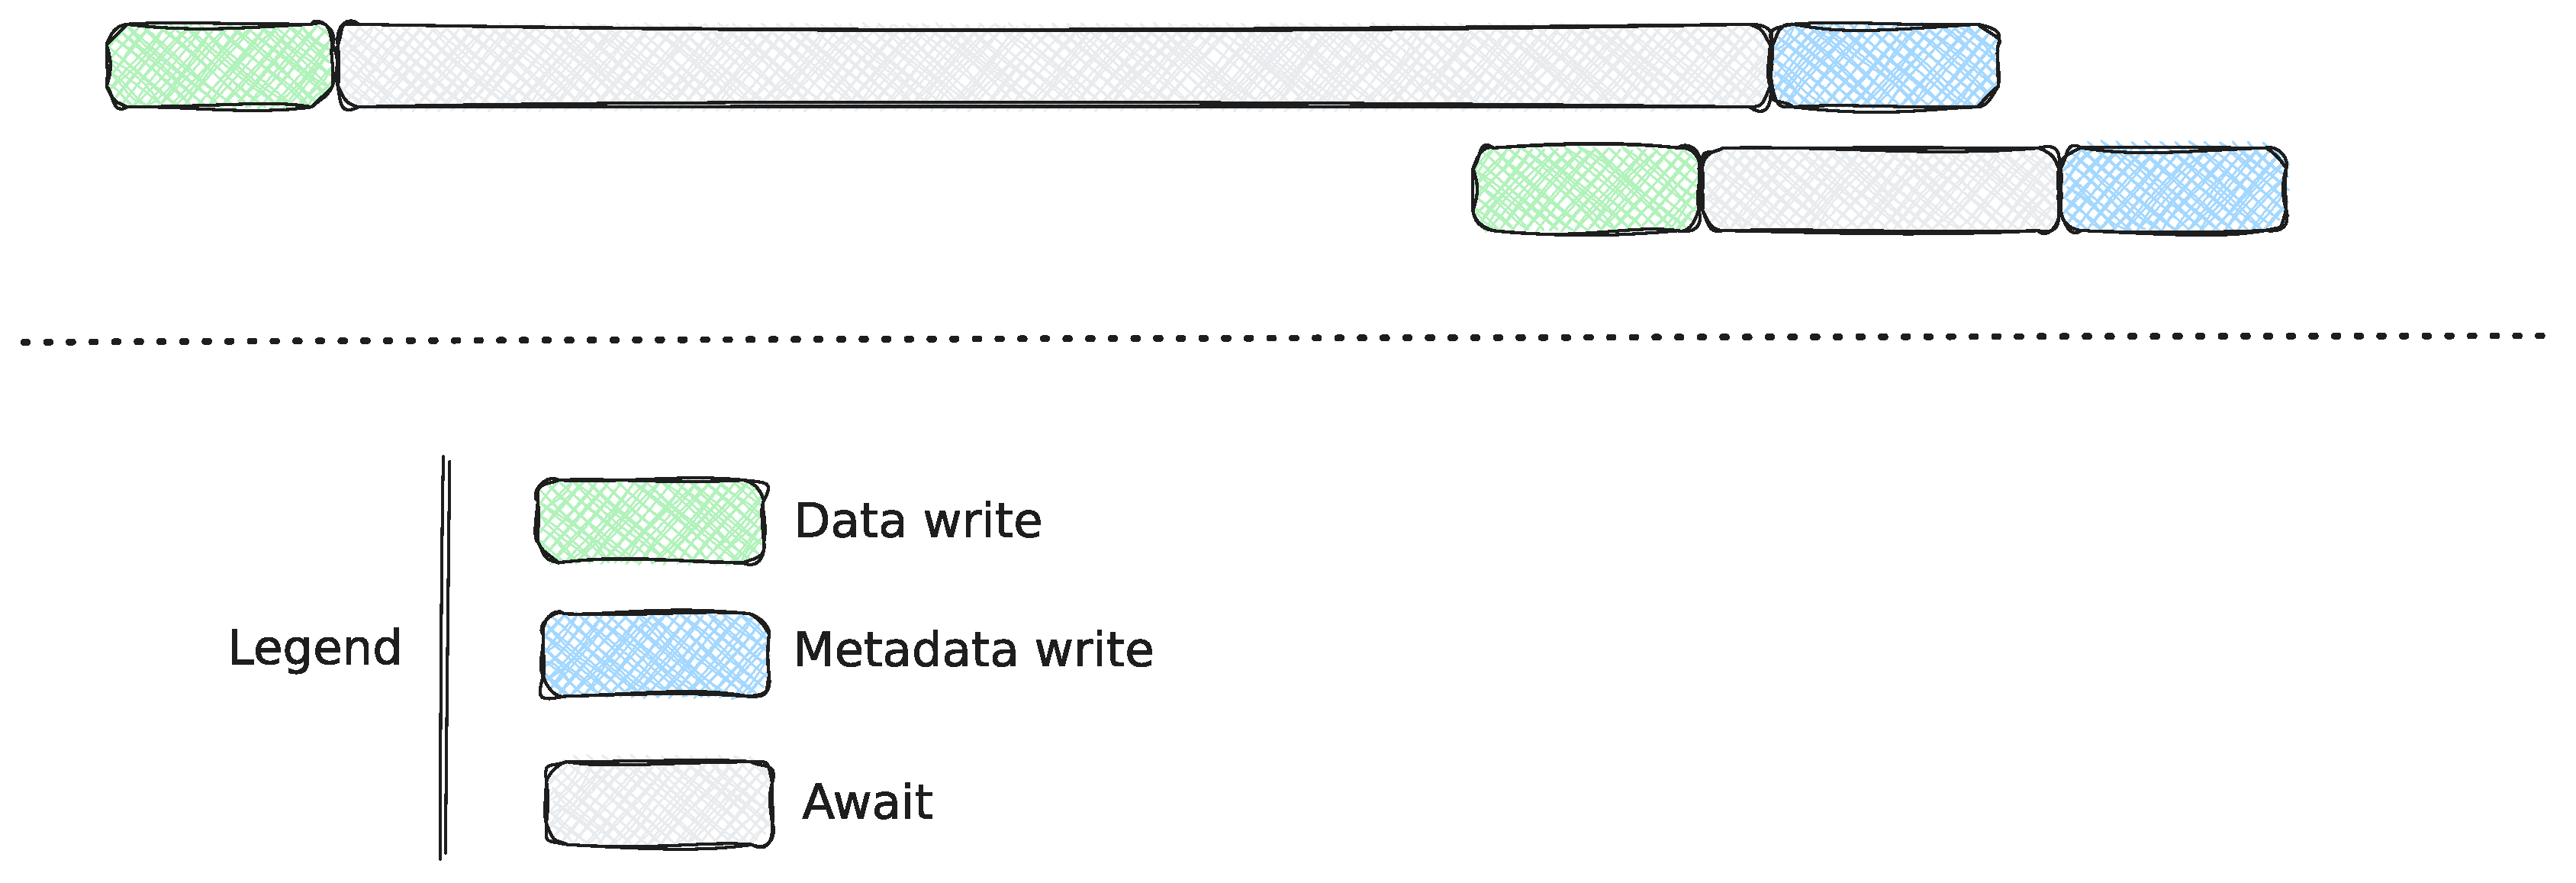
\includegraphics[width=\linewidth]{resources/collision-en}

    In this scenario, a previous migration process may experience significant latency (e.g., a \enquote{stale} or \enquote{zombie} process)
    and be considered timed out by the \textit{Heat} layer, yet remain active and attempt a write after a second migration attempt has already started.
    Transactions are not prohibitive here: a single transaction corresponds to 64\,MiB of data. For a system-wide write throughput of 2\,GiB/s,
    this results in approximately 32 transactions per second—a negligible load for TiKV.

    Furthermore, data persisted in the WAL ensures that a stripe acquired in the current session can be released if the buffer has already been successfully migrated by another process.

    \subsection{Data Compaction and Garbage Collection (GC)}

    \subsubsection{Stripe Compaction}

    Stripe compaction involves reassembling $N$ existing stripes into $M$ new stripes, where $M < N$.
    Container metadata must track the following metrics: the amount of unoccupied space (e.g., failed fragment writes during filling or deleted fragments where space is considered free) and the average fragment size on disk.

    \smallskip
    A \textit{naive compaction algorithm} functions as follows:
    \smallskip

    Iterate through the entries of the stripes being compacted and read the fragments into a memory buffer. During this process, if the next fragment exceeds the remaining buffer capacity (where the buffer size equals the Heat layer block size), a new stripe is allocated to store the accumulated data.

    A \textit{non-naive approach} is slightly more complex, involving fragment reordering and managing multiple buffers simultaneously to achieve optimal filling density for each.

    Overall, this is a straightforward algorithmic task. Naturally, we log intents in the WAL during the process to track stripe states in case of a retry. Upon successful repacking (or immediately after a buffer is saved to a stripe), we perform a metadata update to point \textit{Fragments} to the new locations.

    \subsubsection{Garbage Collection}
    This is perhaps the most challenging topic. As established above, cleanup is performed by reclaiming fragments that are no longer referenced. This is primarily relevant for systems with deduplication enabled. Without deduplication, GC is trivial and can be implemented via a background scan of tuples in cold storage, processed tuple by tuple.

    \smallskip
    Fragments are eligible for deletion when no references to them remain in the \textit{Links} collection. Determining this state directly is computationally expensive:
    \begin{itemize}
        \item \textbf{Maintaining a reverse index} (\texttt{fragment.id} $\rightarrow$ \texttt{record.id, fragment\_index}): While functional, this places a massive burden on the database. It would require $O(1)$ overhead relative to the size of \textit{Links}, which is our largest collection. However, this might be feasible for relatively small-scale installations.
        \item \textbf{Full scan of \textit{Links}}: Heavy and unreliable; shard availability during a full database scan is not guaranteed. This is also only viable for small installations.
        \item \textbf{Reference counting and Access Time tracking}: A more robust approach where $\operatorname{refcount} \leq 0$ combined with a long period of inactivity strongly suggests a fragment is orphaned. However, this requires frequent metadata updates (though this can be optimized—e.g., updating the \enquote{last read} time only once every 24 hours).
    \end{itemize}


    Each of the aforementioned variants has significant drawbacks. It can be argued that the first two are strictly unsuitable for \enquote{exascale} deployments. However, for massive datasets, a typical \enquote{exascale} approach involving offline processing can be applied. This involves emitting events for record creation and fragment-to-record \enquote{linking} to an external analytical store. Possible targets include ClickHouse or storage used by Spark/Flink (in practice, events would be streamed into Kafka or RedPanda and then ingested into ClickHouse).

    \smallskip
    For instance, in ClickHouse, record creation can be represented as \texttt{(datetime, record.id, 1)} and deletion as \texttt{(datetime, record.id, 0)}, with \texttt{record.id} serving as the primary key. By utilizing the \texttt{CollapsingMergeTree} engine, the first entry is effectively replaced by the second once the latter is added.

    \smallskip
    We can then perform a \texttt{LEFT OUTER JOIN} with the table representing \textit{Links} on \texttt{record.id} where \texttt{flag = 1}. If a record has been deleted, its \texttt{record.id} will be \texttt{NULL} for the corresponding entries in \textit{Links}. This allows us to identify fragments eligible for deletion. Specifically, a fragment \enquote{downgrade} approach is proposed:

    \begin{enumerate}
        \item A newly created fragment starts in the \texttt{LIVE} state.
        \item A \texttt{LIVE} fragment identified for deletion transitions to the \texttt{DYING} state. This state is marked by the addition of a \texttt{death\_time} field.
        \item A \texttt{DYING} fragment identified for deletion is finally purged if the current time exceeds the \texttt{death\_time}.
    \end{enumerate}

    \smallskip
    However, this necessitates restricting \enquote{old} fragments from being reused for deduplication. For example, if a fragment matching a hash is older than 3 months, a new fragment should be created, even if it results in a duplicate.

    \bigskip
    This scheme is fully viable provided that data is sent both to the metadata database and to the ClickHouse \enquote{window} during write operations. For example, after writing the record and its fragment links to the metadata DB, the process returns, but the session remains active to asynchronously add the same data to ClickHouse. If the write fails, the session is retried until the data is successfully ingested.

    \subsubsection{Compaction and GC Collisions}

    The previously described logic did not account for potential race conditions. For instance, two concurrent compaction procedures might select the same container and relocate its \enquote{live} content into different target containers. This results in an \textbf{orphaned fragment}:
    \begin{enumerate}
        \item Compaction \#1 updates the reference for fragment $fid$, moving it from the current stripe $A$ to a newly created stripe $B$.
        \item Compaction \#2 performs the same operation, changing the reference from $A$ to stripe $C$.
    \end{enumerate}
    As a result, the system loses track of the fact that stripe $B$ contains fragment $fid$, even though the space it occupies is marked as used. This leads to a \textbf{space leak}.

    Similarly, a collision can occur when compaction and GC results overlap. A fragment $fid$ might be relocated to another stripe while a GC process simultaneously attempts to delete it. The sequence of events could unfold as follows:
    \begin{enumerate}
        \item The GC process identifies which container holds the fragment.
        \item The GC process updates (decrements) the free space counter for that container.
        \item Compaction updates the fragment's reference to point to a new stripe.
        \item The GC process deletes the fragment entry from the \textit{Fragments} collection.
    \end{enumerate}
    Consequently, the container holding the repacked data will store inaccurate information regarding its free space.

    While these issues could be addressed using transactions, the overhead might be prohibitive. Instead, all such collisions can be avoided by ensuring that no two compaction procedures overlap, and that no compaction process runs concurrently with the application of GC results. I propose the following approach:


    \begin{itemize}
        \item A \textbf{task queue} is established to hold compaction and deletion tasks. A message broker is the simplest implementation for this.
        \item A \textbf{Compaction Scheduler} service is created to enqueue compaction tasks.
        \item A \textbf{GC Adapter} service is created to receive data from the GC process and prepare deletion tasks.
    \end{itemize}

    Upon receiving a task, a worker first attempts to acquire a \textit{lease}. The lease is a record in TiKV structured as $high \rightarrow (low, high)$. This acquisition is performed within a transaction:

    \begin{enumerate}
        \item Search for a $lease'$ with the minimum $high' \geq high$. If $low' \leq low$, a collision is detected. The task is rescheduled for a later retry, and no lease is created.
        \item Otherwise, the lease is created, and task execution begins.
        \item \textbf{No TTLs are used.} Using a TTL could lead to a situation where data has been migrated, but metadata updates are only partially complete. Allowing a new process to work on unfinished data could create orphaned resources—occupied containers that are neither referenced nor marked as free. Since operations are performed under a \textbf{WAL}, the system will eventually replay the changes to completion and release the lease upon finalization.
    \end{enumerate}

    \textbf{Compaction task scheduling:} The service iterates through storage regions, partitioning each into segments of random lengths within a specified range. If the last segment of a region is smaller than the minimum allowed size, it encompasses a sub-range of the subsequent region. Crucially, only sub-ranges with indices greater than the current maximum are considered, as regions may change \enquote{under the hood} during the process. The set of regions is treated as a circular buffer, where the \enquote{next} region for the last one is the first region in TiKV.

    \textbf{GC Adapter logic:} This service reads the output from ClickHouse to retrieve fragment identifiers for \enquote{downgrading}. It identifies the regions containing the relevant containers and groups fragments by region. Regions are further divided into uniform sub-ranges to balance the number of tasks against the \textit{lease} range size: more tasks necessitate smaller ranges to minimize lease duration and task weight. For optimal efficiency, the ClickHouse output should be sorted by fragment index in ascending order.


    \newpage


    \section{System Invariants}

    This section defines the properties that must remain true under all operational scenarios, including failures, WAL session retries, and migrations. States that exist only within the scope of specific execution algorithms (e.g., $Hot \rightarrow Migrating \rightarrow Cold \rightarrow Compacted$ for a container) are intentionally excluded. These transient states are not part of the system's core data model and may evolve with the implementation. The invariants focus solely on the verifiable properties of the persistent state, which are sufficient to guarantee data integrity and availability.

    \subsection{Referential Integrity Invariants}

    \paragraph{I1. Single Source of Truth for Placement.}
    The physical location of a fragment is determined exclusively via the following chain:
    \[
        Fragments[fragment.id].container.id \rightarrow Containers[container.id].ref
    \]
    No other collections contain authoritative information regarding physical placement.

    \paragraph{I2. Deterministic Container Placement.}
    For any $container.id$, the $ref$ value must belong to exactly one of the following states:
    \[
        ref \in \{ Hot(hot.id, block.index),\; Tuple(tuple.id, stripe.index)
    \]

    Intermediate or dual states in the metadata are prohibited. The $ref$ must point to a tuple and stripe that exist within the $Tuples$ collection and the allocator's bitmap.

    \paragraph{I3. Single-Fragment Record Integrity.}
    The composition of a $record.id$ in \textit{single} format is defined solely by the fragment identifier stored in $record.single(fragment\_id)$.

    \paragraph{I4. Multi-Fragment Record Integrity.}
    The composition of a $record.id$ in \textit{multi} format is defined exclusively by the following mapping in the \textit{Links} collection:
    \[
        (record.id, fragment.index) \rightarrow fragment.id
    \]
    The \textit{Records} collection does not contain authoritative information regarding the composition of records in \textit{multi} format.

    \paragraph{I5. Fragment Immutability.}
    After a record is committed, the following fields:
    \[
        (offset,\; size,\; crc64,\; compression,\; blake3)
    \]
    must remain immutable.любое Any change to the content necessitates the creation of a new $fragment.id$.

    \paragraph{I6. Tuple Integrity.}
    For any $tuple.id$ in \textit{Tuples}, the number of disks in the $disks$ array and their respective roles must strictly conform to the scheme defined in $type$.

    \subsection{Hot $\rightarrow$ Cold Migration Invariants}

    \paragraph{M1. Migration Completion via Reference Swap.}
    A container migration is considered complete only after an atomic replacement:
    \[
        Hot(\cdot) \rightarrow Tuple(\cdot)
    \]
    within $Containers.ref$.

    \paragraph{M2. Stripe Commitment Condition.}
    A stripe is considered occupied (\textit{Committed}) only after:
    \begin{enumerate}
        \item Successful write operations for all blocks.
        \item Successful atomic update of $Containers.ref$.
    \end{enumerate}

    \paragraph{M3. Stripe Write Exclusivity.}
    Writing to $(tuple.id, stripe.index)$ is permitted only under an active Lease issued by the RAFT allocator. A lease for $(tuple.id, stripe.index)$ is granted only if the disk configuration in \textit{Tuples} allows for the write operation (e.g., all required disks are healthy and accessible).

    \paragraph{M4. Migration Idempotency.}
    If $Containers.ref$ already points to a $Tuple(\cdot)$, any migration retry must complete without side effects.

    \paragraph{M5. Reference Swap Constraints.}
    An atomic transition is only possible as $ref\_expected \rightarrow Tuple(\cdot)$, where $ref\_expected$ is the exact current value of $Containers.ref$ (must be a $Hot$ or composite $Hot$ state, i.e., not $Cold$).

    \subsection{WAL and Retry Invariants}

    \paragraph{W1. WAL Enforcement for Multi-Step Operations.}
    Any operation spanning more than one domain (Heat, Cold, or Metadata) must be executed within a WAL session.

    \paragraph{W2. Duplicate-Free Retries.}
    The retry of a WAL session must not create additional references, stripes, or containers. A retry operation must either:
    \begin{itemize}
        \item Overwrite the existing values with the same data,
        \item Or detect a finalized state and terminate execution.
    \end{itemize}

    \subsection{Deduplication and GC Invariants}

    \paragraph{D1. Dedup only affects fragment.id selection.}
    Deduplication does not alter the reference model. Connections between a record and its fragments are always expressed via the $Links$ collection.

    \paragraph{G1. Fragment deletion is only permitted in the absence of references.}
    A fragment may be deleted if and only if there are no rows in $Links$ pointing to the given $fragment.id$.

    \subsection{Execution Invariants}

    \paragraph{E1. Writing to stripe blocks and buffers is only possible with an active Lease.}
    Any write operation to a cold stripe or a hot buffer is permissible only if a valid $lease.id$ exists, issued by the corresponding coordinator (RAFT allocator or hot node). If the Lease is lost or expired, write operations must become impossible.

    \subsection*{4.X. Ownership and Concurrent Execution Invariants}

    \paragraph{O1. Single range owner.}
    In any given moment, there is no more than one process with the right to modify containers within range $R$. This right is determined by a valid $lease.id$ issued by the Range Manager.

    \paragraph{O2. Container modification only via range queue.}
    Any operation that changes the state of a container (including fragment redistribution, updates to free space metrics, compaction results, or GC) is performed exclusively as a task in the queue of the corresponding range by its owner.

    \paragraph{Q1. Linearizability of range task execution.}
    Range tasks are executed sequentially by a single executor. Each task has a unique identifier $(rangeID, taskID)$. Re-submission or re-execution of a task does not violate correctness (ensured via idempotency or duplicate execution detection).

    \paragraph{Q2. Monotonicity of progress.}
    For each range, there is a monotonic progress point $ack$. The $ack$ value can only move forward. Recovery after a restart is performed by resuming from the last recorded $ack$.

    \paragraph{G2. GC injection relevance.}
    When applying an $\mathrm{InjectGC}(container, F)$ task, for each $f \in F$, the action is permissible only if, at the time of execution:
    \[
        \mathrm{Fragments}[f].container\_id = container.
    \]
    Otherwise, the operation is a \emph{no-op}.

    \paragraph{G3. No direct GC writes to containers.}
    The GC process does not perform direct modifications to the container structure. It only generates range tasks, which are then executed by their respective owners.

    \paragraph{M6. Placement persistence before resource commit.}
    Any commit of a cold-layer resource is permissible only after a successful atomic transition:
    \[
        ref_{expected} \rightarrow Tuple(\cdot),
    \]
    executed within a transaction. If the transition fails, the resource is not committed.

    \paragraph{ID1. Canonical key identifier.}
    In all structures requiring uniform distribution, the following key is used:
    \[
        id_{key} = \mathrm{SPECK}_{128}(id_{raw}),
    \]
    where $\mathrm{SPECK}_{128}$ is a bijective permutation. This ensures a statistically uniform distribution of containers across ranges.


    \newpage


    \section{Supplementary Materials}

    \subsection{Complete WritePath for multiple fragments}

    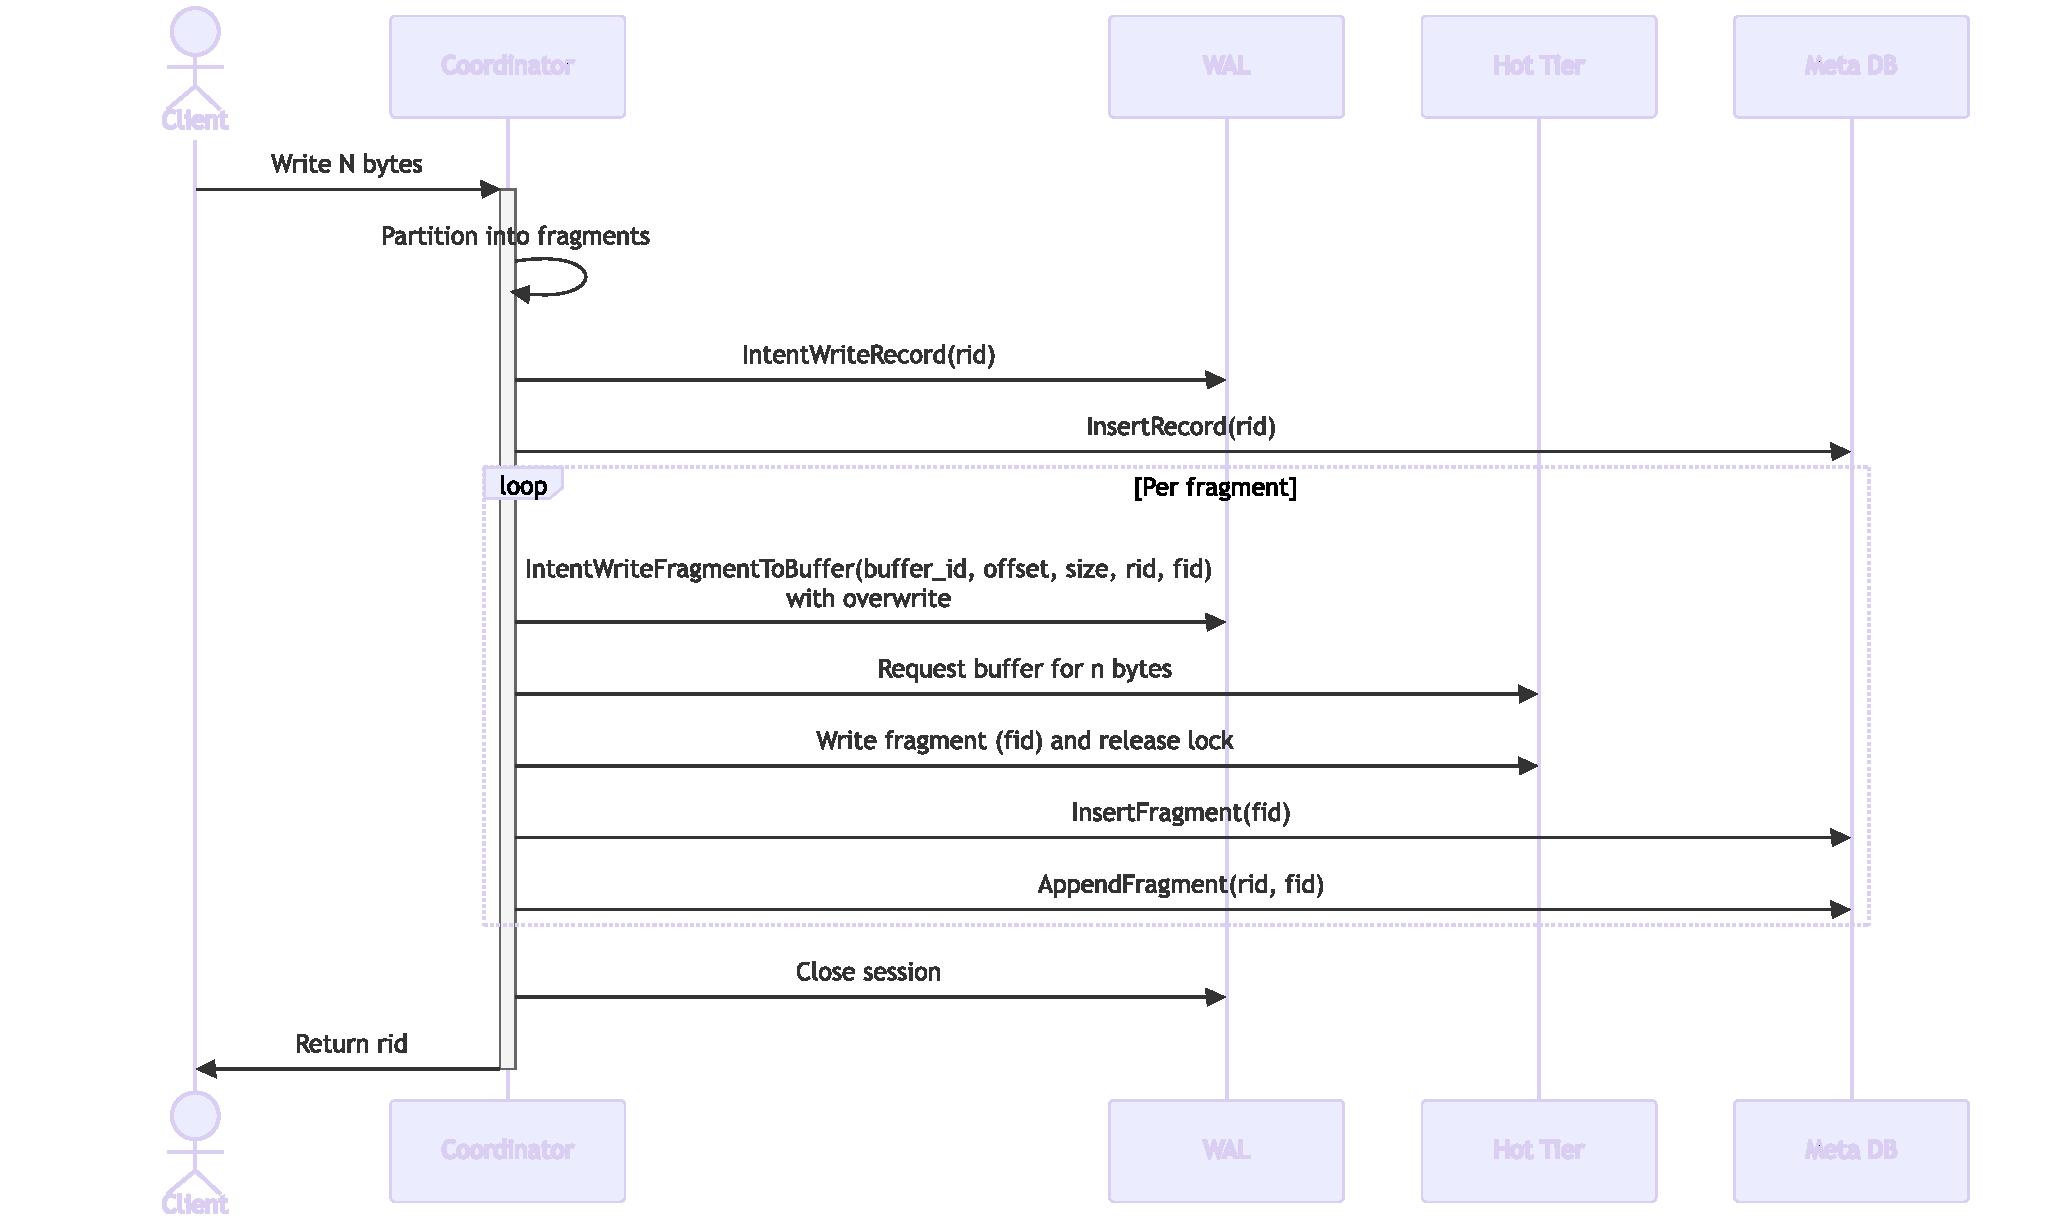
\includegraphics[width=\linewidth]{resources/write-path-multi-hot-en}

    The advantage here is that database operations do not need to be transactional; invariants are ensured by the WAL and the idempotency of the logic.

    \subsection{Complete MultiWrite}

    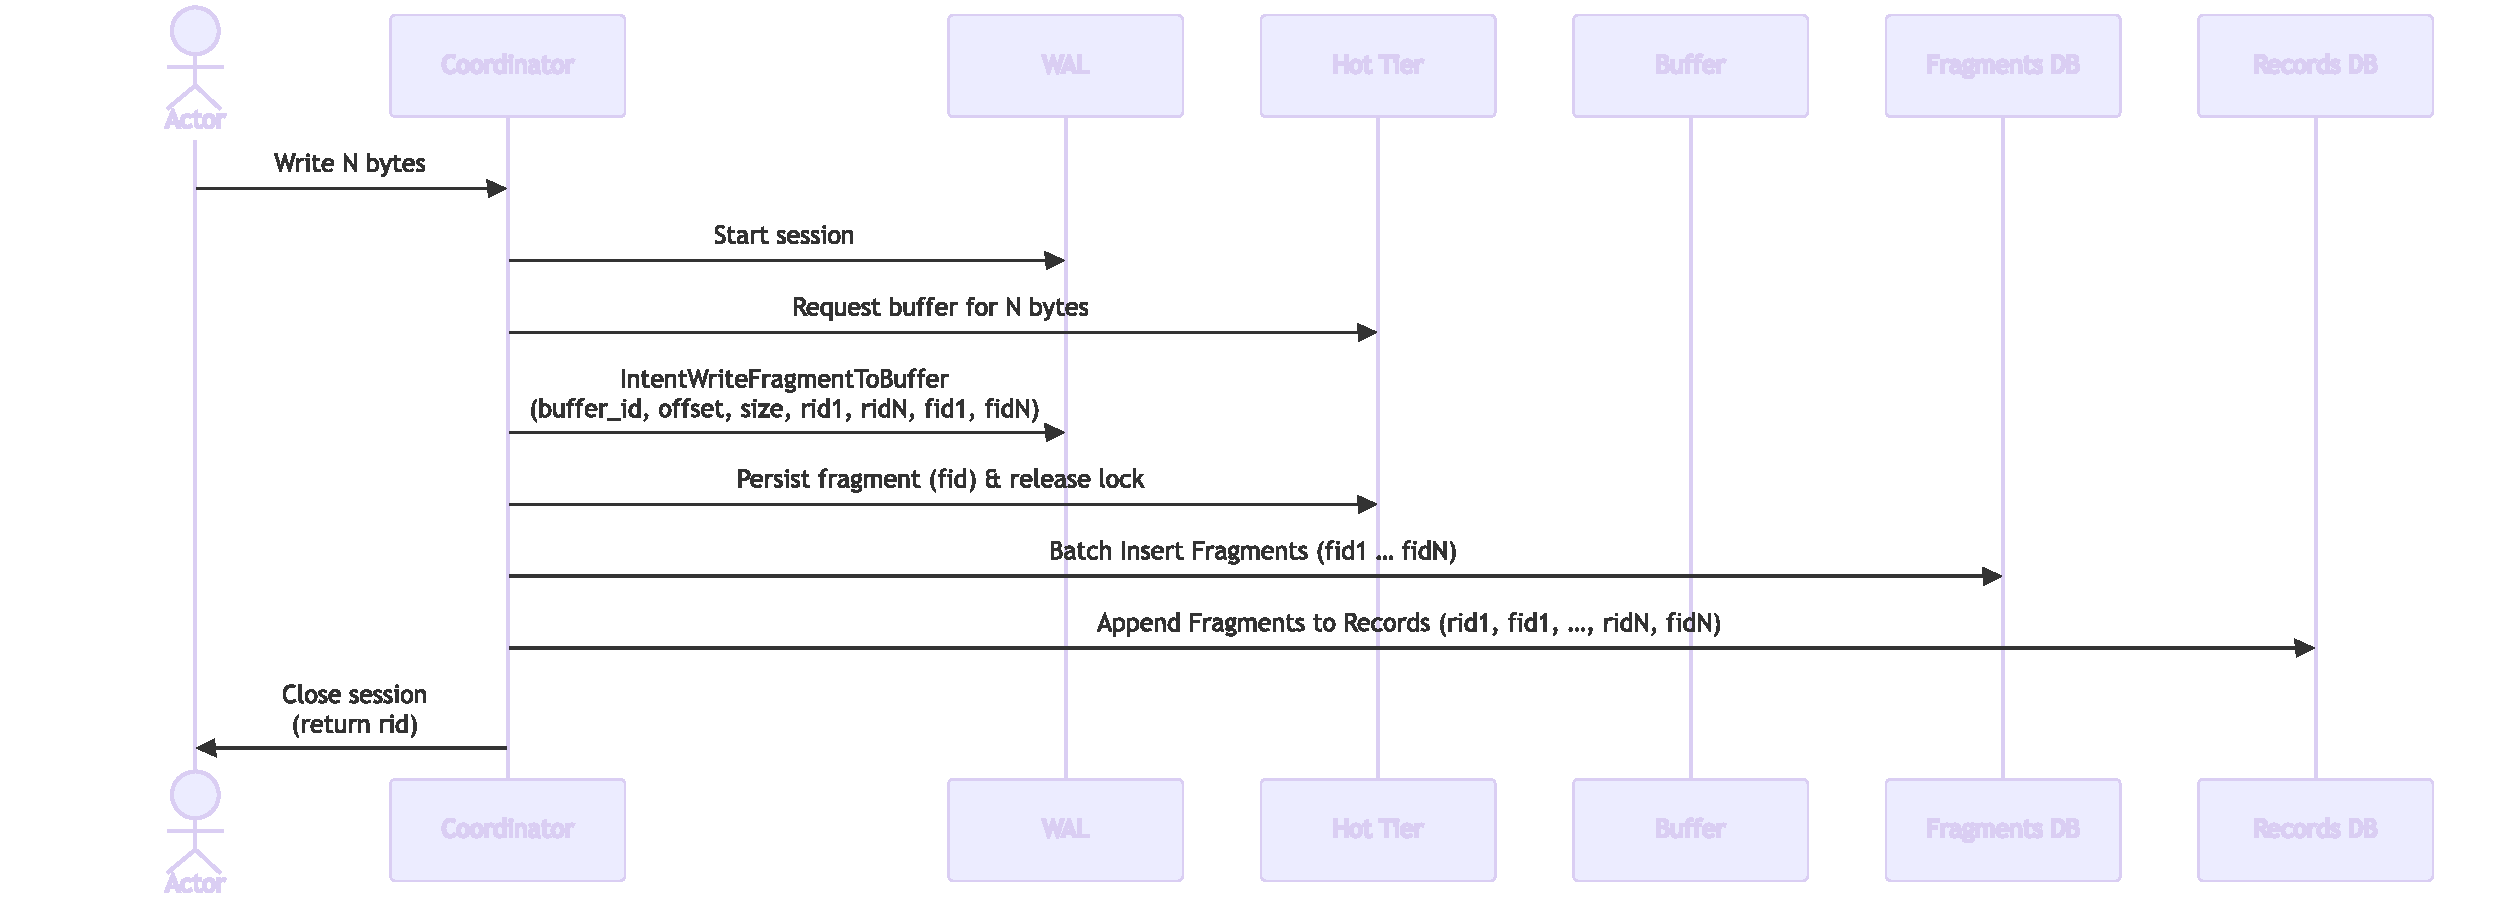
\includegraphics[width=\linewidth]{resources/multi-write-en}

    Inserting multiple fragments simultaneously. This process is critical for system performance when inserting small data chunks. Such operations place a high load on the meta-layer due to the massive influx of records. The scheme described here reduces the load on the WAL by using ranges ($rid_1, rid_N$) and ($fid_1, fid_N$) to store intents. It also alleviates pressure on the metadata storage through the use of batch writes.

    Please note that "original" identifiers are used for $rid_1 \dots rid_N$ and $fid_1 \dots fid_N$ instead of their $\mathrm{SPECK}_{128}$ values. This is done specifically to enable range notation rather than exhaustive enumeration. In the event of session errors, the recovery process will, of course, operate with transformed values. That is, when verifying $rid_K$ from the $[rid_1 \dots rid_N]$ range, we are actually checking the record with the identifier $\mathrm{SPECK}_{128}(rid_K)$.

    \subsection{On WAL implementation using a message broker and KV storage}

    A distributed WAL is implemented, maintaining one log per session. The following operations are available within a session:

    \begin{itemize}
        \item Add data – Append.
        \item Overwrite data – Overwrite.
        \item Close session.
        \item Retry session with a delay of at least $T$ seconds.
    \end{itemize}

    It is proposed to implement these operations using a message broker and a KV store. NATS + JetStream is suggested as the broker. For the KV store, any persistent solution will work; In-Memory storages like Tarantool or Redis are best suited among persistent options. For disk-based solutions, Aerospike is a strong candidate.

    LSM-based storages using RocksDB under the hood are strictly unsuitable. This is because our workload implies:

    \begin{itemize}
        \item Continuous creation of new records with no repeating identifiers.
        \item Deletion of the vast majority of records within a fraction of a second.
        \item Most records that survive those initial fractions of a second will still be deleted within seconds.
    \end{itemize}

    In these conditions, the skip list in RocksDB (which stores the in-memory LSM table) is highly suboptimal due to its lazy deletion nature. It would lead to extreme IO overhead (write amplification) during subsequent compactions.

    \subsubsection{Introduction}

    Upon session initialization, the coordinator receives a fresh session\_id (hereafter referred to simply as $id$), which is 16 bytes (128 bits). Under these conditions, we define:

    \[K = \operatorname{big\_endian}(id)\]
    \[K' = \operatorname{append}(K, 0)\]

    That is, a zero byte is simply appended to $K$ to form $K'$.

    \subsubsection{Working with KV storage}

    At the start of the operation, a background process is immediately launched to periodically write the current \texttt{unixtime} to $K'$ with an established $\text{TTL} = T$. This is done at an interval of, say, one second; higher frequency is unnecessary. The session data is structured as follows:

    \begin{center}
        \begin{tabular}{|l|r|}
            \hline
            header & data \\
            \hline
        \end{tabular}
    \end{center}

    The header includes, among other things, the count of retries performed for this session, while the data is a sequence of binary chunks in the following format:

    \begin{center}
        \begin{tabular}{|l|c|c|c|c|c|r|}
            \hline
            varint(len1) & data1 & varint(len2) & data2 & \dots & varint(lenN) & dataN \\
            \hline
        \end{tabular}
    \end{center}

    All session binary data is always held by the coordinator. Under these conditions:

    \begin{itemize}
        \item The \textbf{Append} operation corresponds to adding a new \texttt{varint(len(data)) + data} to the session data, followed by writing the entire payload (including the header) into the value associated with key $K$.
        \item The \textbf{Overwrite} operation corresponds to deleting all data following the header, adding a new fragment, and subsequently writing the result.
    \end{itemize}

    When a session completes successfully, the value $K$ is deleted from the database. If the session fails, we simply exit. A failure to update $K'$ is considered a session operation failure.

    \subsubsection{Working with the broker}

    All coordinators are subscribed to a specific broker topic. Event distribution is not broadcast; instead, messages are delivered to only one of the subscribers (competing consumers pattern).

    \smallskip
    An event containing only $K$ is sent to this same topic, with an instruction to deliver it no earlier than after $T$ seconds (delayed delivery).

    \smallskip
    Upon receiving an event, the process follows one of these scenarios:

    \begin{itemize}
        \item There is no record with key $K$ in the database. This indicates the session has been completed. Ack.
        \item The value in $K'$ was updated too recently (the timestamp is still fresh). Request redelivery after $T$ seconds.
        \item The retry counter in record $K$ has exceeded the limit. Log the error, delete $K$, and send an Ack.
        \item None of the above conditions are met. Initiate session recovery by starting the $K'$ updater, increment the retry counter by one (persisting the new value immediately), and resume operations based on the data recorded in the session. From this point, the process follows the steps described in the \enquote{Working with KV} section.
    \end{itemize}


    \section{Specialized WAL Solution}

    A Push-Push interaction variant is proposed, operating as follows:

    \subsection{Consensus Node}

    The WAL consensus node consists of $2n + 1$ machines running MultiRAFT or a similar consensus protocol. It maintains $2n + 1$ internal RAFT instances, where each host acts as the leader for one instance and as a follower for the others.

    Each host implements an interface of the following type:

    \begin{lstlisting}
rpc Session(stream SessionReq) returns (stream SessionResp)

type SessionReq oneof {
  Init(clientClass) // Only the first message in the stream.
  Append(bytes)
  Overwrite(bytes)
  Close             // Only the last message in the stream.
  Repeat(T seconds) // Only the last message in the stream.
  Pulse             // Can occur anywhere in the stream.
}
    \end{lstlisting}

    \texttt{SessionResp} contains acknowledgments for the performed operations; each response is expected synchronously.

    The client connects to a \textbf{specific} host of such a node and initializes it using \texttt{Init}, then executes a sequence of \texttt{Append}/\texttt{Overwrite} operations and finishes with a final \texttt{Close}/\texttt{Repeat}. Meanwhile, a \texttt{Pulse} (also acknowledged) is periodically sent in the background.

    Active sessions are stored in memory. Sessions scheduled for retry are stored in an LSM-tree, ordered by retry time:

    \begin{center}
        \begin{tabular}{|l|c|r|}
            \hline
            repeat\_time & headers & data \\
            \hline
        \end{tabular}
    \end{center}

    If a client disconnects, the session is sent for retry. If a host fails, the former follower that becomes the new session leader immediately sends the active sessions of the inherited RAFT instance for retry. Session retries are initiated via consensus.

    \subsection{Clients}

    Services responsible for processing session retries must implement an almost mirror-symmetrical interface:

    \begin{lstlisting}
rpc SessionRepeat(stream SessionRepeatReq) returns (stream SessionRepeatResp)
    \end{lstlisting}

    Where \texttt{SessionRepeatResp} looks almost exactly like \texttt{SessionReq}, while \texttt{SessionRepeatReq}
    includes a new branch compared to \texttt{SessionResp}:

    \begin{lstlisting}
type SessionRepeatReq oneof {
  Deliver(session_headers, session_data) // Only the first in the stream.
  // Further fields are identical to SessionResp.
}
    \end{lstlisting}

    During a retry, the node host identifies the class of services required for the session retry and connects to them for execution, starting with the delivery of the session data. This constitutes the second "Push" in the \enquote{Push-Push} scheme.

    \newpage


    \section{Roadmap}

    \subsection{MVP}

    \begin{enumerate}
        \item Implementation of the RAFT allocator.
        \item Implementation of a service providing access to machine disks on JBOD using Go and io\_uring.
        \item Tuples implementation and refinement of the logic for binding disks to a tuple (considering that the host machine may change).
        \item Testing block uploads to a "cold node."
        \item Implementation of the selected hot storage host type using Go + io\_uring.
        \item Implementation of a hot storage node.
        \item WAL scaffolding and integration.
        \item Consolidation of metadata logic and final database selection.
        \item Implementation of the coordinator.
    \end{enumerate}

    \subsection{GC}

    Research GC implementations for small-scale installations and for "exascale" using Clickhouse via Kafka as a sidecar process.

    \subsection{Logic Evolution}
    \begin{enumerate}
        \item Grouping tuples in the allocator by redundancy types. This allows the allocator to consider only those tuples configured for a specific Erasure Coding (EC) or replication scheme.
    \end{enumerate}

    \subsection{Optimization}
    \begin{enumerate}
        \item Implementation of a hot storage host with NVMe and NVDIMM using SPDK (selecting either C or Rust).
        \item Implementation of JBOD-based nodes in Rust using io\_uring.
        \item Replacing the placeholder NATS + JetStream WAL with a specialized multi-master Push-Push WAL.
        \item Introduction of an archival layer where data and metadata are compressed within a single container, while TiKV stores only Bloom filters and coordinates of the archival layer's tuples and stripes. Data layout in stripes is identical to the cold layer but utilizes smaller EC schemes (in terms of $P$) and larger stripe sizes (e.g., 1 GiB instead of 64 MiB). This will alleviate the load on TiKV, which may otherwise struggle with a high volume of small records where metadata weight approaches the weight of the actual data.
        \item \textbf{High-throughput "Pipes" for small objects.}
        Introduction of an asynchronous ingestion mechanism for small-scale data. In this mode,
        data is buffered directly to SSD/NVDIMM without immediate metadata registration.
        The system provides a post-write callback to bind external identifiers to the
        resulting \texttt{record.id} set, significantly reducing pressure on the metadata layer.

    \end{enumerate}

    \subsection{Description of the \enquote{Continuation} Mechanism}

    During streaming, a buffer may fail. In this case, the system can look for another buffer elsewhere and resume writing not from the beginning, but from the position where the recording on the failed buffer was interrupted. During the transfer process, the first and second buffers are "stitched" together at the break point. This transition is, of course, reflected in the metadata.

\end{document}
